\documentclass[paper=a4, fontsize=11pt]{scrartcl}
\usepackage[T1]{fontenc}
\usepackage{fourier}

%\usepackage[english]{babel}															
\usepackage[english]{babel}
\usepackage{indentfirst}		% for indent
\usepackage[utf8]{inputenc}


\usepackage[protrusion=true,expansion=true]{microtype}	
\usepackage{amsmath,amsfonts,amsthm} % Math packages
\usepackage[pdftex]{graphicx}	
\usepackage{url, array}
\usepackage[num,abnt-repeated-author-omit=yes]{abntex2cite}


%%% Custom sectioning
\usepackage{sectsty}
\allsectionsfont{\centering \normalfont\scshape}


%%% Custom headers/footers (fancyhdr package)
\usepackage{fancyhdr}
\pagestyle{fancyplain}
\fancyhead{}											% No page header
\fancyfoot[L]{}											% Empty 
\fancyfoot[C]{}											% Empty
\fancyfoot[R]{\thepage}									% Pagenumbering
\renewcommand{\headrulewidth}{0pt}			% Remove header underlines
\renewcommand{\footrulewidth}{0pt}				% Remove footer underlines
\setlength{\headheight}{13.6pt}


%%% Equation and float numbering
\numberwithin{equation}{section}		% Equationnumbering: section.eq#
\numberwithin{figure}{section}			% Figurenumbering: section.fig#
\numberwithin{table}{section}				% Tablenumbering: section.tab#


%%% Maketitle metadata
\newcommand{\horrule}[1]{\rule{\linewidth}{#1}} 	% Horizontal rule

%\date{\today}

%%% Begin document
\begin{document}
		
{\flushleft\horrule{2pt}
\begin{center}
{
\includegraphics[height=0.09\textwidth]{Figs/logo_english.png}} 
\begin{tabular}{ m{1.8cm} m{10cm} m{1.8cm}}
\begin{center}
\end{center}
&
\begin{center} 
{\small
{Adrar University} \\
{Faculty of Science and Technology} \\
{Department of Mathematics and Computer Science}} \\

\end{center}
&

\begin{center}
\end{center}
\end{tabular}
\end{center}
\flushleft \horrule{2pt}\\[1cm]
}


\begin{center}

{
\huge  
Initiation to Research (Course) \\
\vspace{0.2cm}
2\textsuperscript{nd} Year Master (S3) \\
\vspace{0.2cm}
2020/2021}\\

\vspace{1cm}

{
\Huge   
\textbf{Build a parallel corpus (Algerian Dialect,  Modern Standard Arabic) and apply Deep Neural Machine Translation on it }}\\
\vspace{1cm}

%Domain: Mathematics and Computer Science \\
%Major: Informatics - Intelligent Systems \\
{
\Large
\textbf{Elwannas HIRI \footnote{Email: hiri.elwannas@gmail.com}}}\\
\vspace{3cm}

{
\large
\textbf{Instructor: Dr. Abdelghani DAHOU \footnote{Email: dahou.abdghani@univ-adrar.edu.dz}}}\\
\today
\end{center}
\pagebreak
\tableofcontents
\pagebreak
\listoffigures
\pagebreak






\section{Abstract}
Arabic Dialects are getting under search radar lately, especially in the Artificial Intelligent (AI) field, the last one requires a huge amount of data to learn from it. Modern Standard Arabic used in official newspapers, Conferences,  books and more. On the other, hand we have various dialects. Some of them are similar to the Moroccan dialect(MD) and some of them are similar to Tunisian dialects(TD) and the others are just Algerian original dialects. In this research proposal, we first present how we built a 13,000 parallel  Algerian Dialects(AD) to Modern Standard Arabic(MSA) sentences. Next, we present our first experiment using FAIRSEQ\cite{ott2019fairseq} toolkit on our data set, and why we used FAISEQ\cite{ott2019fairseq} instead of others\cite{zhang2015deep}. The first experimental results was 1.02 using the BLUE4 Score without any modification on the data set. Finally a short description of future work to get a better result.

\section{Introduction}
Sentences for each file, we had created a help post in Facebook help community, also posted in 1001Tech\footnote{Facebook Group: https://www.facebook.com/groups/dztech1001/} group, received 126+ files from all the Algeria regions. To boost the process we paid 4 people to write 6400 sentences. After collecting the data and organize it we got 14,000 sentences (until 14-02-2021). Since 2010, several works are using Statistical Machine Translation(SMT), SRILM, and Other approaches such as machine translation system that uses an MSA pivot approach\cite{meftouh2015machine}. Lately, deep neural networks came to the machine translation field. Many approaches have been developed such as Deep Neural Network(DNN), Feed Forward Neural Network(FFNN), Conventional Neural-Network(CNN), Recursive Neural Network (RNN) and finally Purely Neural Network \cite{zhang2015deep}.  Available DNN toolkits (e.g. Open-NMT\footnote{Open-NMT: A modern toolkit for machine translation}, FAIRSEQ\cite{ott2019fairseq}) are widely used by big companies(e.g. Google Translate, Facebook). The study will help to increase the interaction between Arab countries. In recent years topics like Arabic Dialects are widely discussed in social media, this results increase the attention between Arabs them selves. The main motivation for the creation of parallel corpus is Dial2MSA\cite{mubarak2018dial2msa}, on the other hand the power of current machine translation is a good motivation for the Machine Translation side. Previous works  \cite{meftouh2015machine}  \cite{tachicart2014hybrid}  \cite{mahgouba2015translator} used up in years methods. We took the state of the art which is FAIRSEQ\cite{ott2019fairseq}, we applied Transformer model on our data set, we got a 1.02 BLUE4 score for the first experiment. For the future work, we are going to extend the data using some methods, normalize data and try to get better results.
\section{Related Works}

\subsection{PADIC\cite{meftouh2015machine}}
PADIC\cite{meftouh2015machine} is a 6,400 sentences corpus of five different dialects Annaba(Algerian city), Algiers(Algeria Capital), Palestinian, Tunisian and Syrian Dialects with MSA parallel sentences. Algerian Dialect is non-resourced language. The PADIC corpus was built from scratch. Using Kneser-Ney and Witten-Bell smoothing techniques the BLUE results gotten  from translating AD to MSA were respectively 15.1, 14.64. Sentences was written in Transliteration\cite{meftouh2015machine}. 
\subsection{Dial2MSA \cite{mubarak2018dial2msa}}
Dial2MSA\cite{mubarak2018dial2msa} was the first multi dialects corpus. The Corpus contains 5500 tweets written in Egyptian, Gulf, Levantine, Maghribi with MSA translations. Twitter was the source of data, 175M tweets have been filtered with powerful words of the dialects. CrowedFlower\footnote{CrowedFlower website has been changed to: https://visit.figure-eight.com/} was the tool controlling the quality of data annotation\cite{mubarak2018dial2msa}.
\subsection{ "A Translator for Arabic Dialects to Modern Standard Arabic" \cite{mahgouba2015translator}}
The Study \cite{mahgouba2015translator} was about applying Morpho-Semantic analysis, Morphological analyser to obtain the translation.
\subsection{"A hybrid approach to translate Moroccan Arabic Dialect" \cite{tachicart2014hybrid}}
Arabic Dialects are characterized by diglossia\footnote{diglossia: A situation in which two languages (or two varieties of the same language) are used under different conditions within a community, often by the same speakers.}. MGB Dialect uses words from other langauge for example Spanich, French, Amazigh and MSA. By applying the morphological analysis and rule-based translation system with smoothing using statistical tool the performance of translation get better. Sentences were written in transliteration form using Buckwalter.  
\subsection{"An Algerian Dialect study and Resources" \cite{harrat2016algerian}}
This work is a part of TORJOMAN\cite{harrat2014building}, an analysis for Algiers Dialect. The work present Phonological differences, types of verbs, negation form in the Algerian day to day speech, types of particles and Inflection of Algerian Dialect from MSA \cite{harrat2016algerian}.    
\subsection{ "Parallel resources for Tunisian Arabic dialect translation" \cite{kchaou2020parallel}}
A combined work of three corpora of dialects to translate Tunisian Dialect to MSA. The Research was focused on getting the largest possible TD-MSA corpus to apply Machine Translation on the data.Three experiments was tried, the first one got 12 on BLUE score, the result was caused by the difference between vocabulary used in corpora, the last one reach 15.03 BLUE score after the adjustment.

\pagebreak
\section{Methodology/Research Methods}

The workflow of this research is presented below:
\begin{itemize}
    \item Build corpus 
    \begin{itemize}
        \item Split the data set
        \item Distribute it the largest possible regions in Algeria to get more data
    \end{itemize}
    \item Normalizing the data set
    \item Create a vocabulary using subword-nmt\footnote{subword-nmt: Byte Pair Encoding method to create a vocabulary in order to train the data }
    \item Train the data using FAIRSEQ\cite{ott2019fairseq} with Transformer model.
    \item Adjust parameters for better results.
\end{itemize}

Previous presented related works used old methods for Machine Translation. We are entering the AI field on this research. Lately Deep Neural Network entred all research fields like Image processing Speech Recognition...etc. In 2017, Google Translate has used the OpenNMT. All Methods of Deep Learning Neural Network Machine Translation are presented in \cite{zhang2015deep}.

\subsection{Building the Corpus}
Using the free Data set from Tatoeba, we split it into 100 sentences for each excel file to make the translations easier. More than 150 person helped to build the corpus from 22 different cities. Adrar and Tipaza were the most active cities in this translations process. 126 files has been received. .txt,.csv,.xlxs are files types received. everyone can use the corpus after publishing the article.
\subsection{Normalizing the data}
The process of Normalizing the data is simple for the first experiment just removing the numbers, dots, commas and repeated sentences.
\subsection{Create vocabulary using Subword-nmt}
Subword-nmt is the main state of the are used techniques to create the vocabulary before training the data in Deep Neural Network Machine Translation systems. By fixing the vocab to 2000 words, the vocabulary is ready to be used by the model.
\subsection{Train the data set using FAIRSEQ\cite{ott2019fairseq}}
FAIRSEQ\cite{ott2019fairseq} is newest toolkit developed by Facebook under Pytorch library. we choose FAIRSEQ\cite{ott2019fairseq} because of it performance and large support of models in addition tothe ability to online back translation and EM-style\cite{shen2017style} training to produce lower the loss.
\pagebreak
\subsection{Results}
For the model Transformer, we used these parameters: \\
\begin{itemize}
    \item 3 by 3 for the hidden layers
    \item batch 400 
    \item learning rate 1e-3 \\
    \paragraph{}
    Caused by the amount of resources
    \item Drop out 0.01
    \item Adam for smoothing
    \item Token size 200
\end{itemize}
The result we got is 1.02 using BLUE4 evaluation and it is explained by:
\begin{itemize}
    \item Lack of DA resources 
    \paragraph{}
    Neural networks requires a big amount of data to get better results
    \item Different Dialects
    \item Simple Normalization
\end{itemize}

\section{Future Work}
Our Future work is based on:
\begin{itemize}
    \item extending the corpus by adding PADIC\cite{meftouh2015machine},Dial2MSA \cite{mubarak2018dial2msa} , Tunisian Dialect corpus  and Moroccan resources.
    \item Normalizing the data using different available methods.
    \item Try different models than Transformer to our data set.
    \item Try models on our data set based on regions.
\end{itemize}
  



\pagebreak
\section{Project Timeline}
This work has Started from November 22th, 2020 it started by exploiting current researches and techniques. For now it is all about learning availables models , trying normalization methods and adjusting the parameters and getting better results.  Building the corpus takes forever. \\ 


\begin{figure}
    \centering
    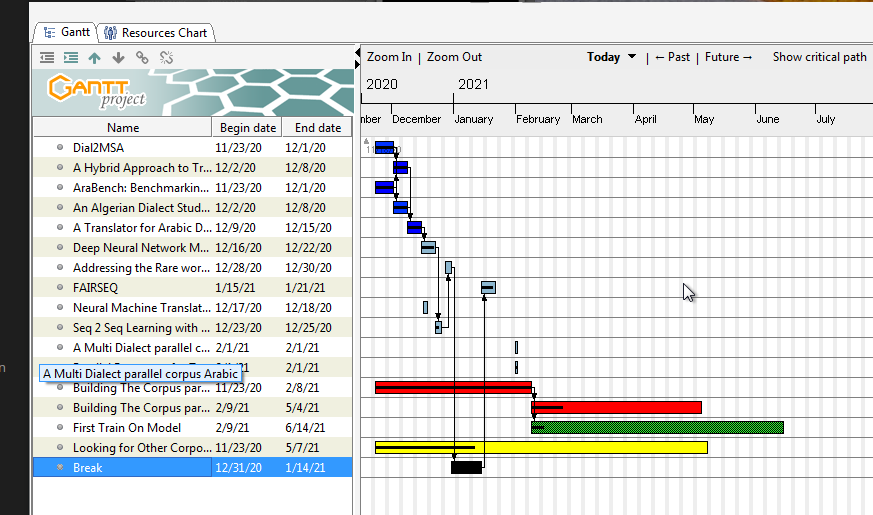
\includegraphics[height=0.55\textwidth]{Figs/dd.png}
    \caption{WorkFlow Time Line}
    \label{fig:my_label}
\end{figure}

\pagebreak
\bibliographystyle{abnt-num}
\bibliography{ref}

\end{document}